\documentclass[letter,12pt]{article}
\usepackage{jheppub}
\usepackage{taro}
\usepackage{booktabs}
\newcommand{\la}{\langle}
\newcommand{\ra}{\rangle}

\title{Notes on integrands for $\mathcal{N}<4$}
\author{Taro Brown}
\date{February 2023}

\begin{document}

\maketitle

\section{Generalized Unitarity}
Loop integrands are rational function and hence may be expanded in arbitrary basis

\section{Loop integrals and momentum twistors}
In general, one-loop amplitudes can be decomposed in terms of a set of basis functions, $I_i$, with coefficients, $c_i$, that are rational in terms of spinor products,
\begin{equation}
	\begin{aligned}
		A= \sum_i c_i I_i
	\end{aligned}
\end{equation}
For $\mathcal{N} = 4$ amplitudes the set can be taken to contain scalar boxes, $I_4$. We have here 4 cases, labeled by whether external momenta are massive or mass-less\footnote{In reality we are always working with massless particles and the notion of \textit{massive} is taken to mean multiple particles in the external lines such that the summed momenta looks like a massive particle, e.g. $(p_1+p_2)^2="m_{12}^2"\neq0$}. The cases that we encounter are:
\begin{figure}[H]
	\centering
	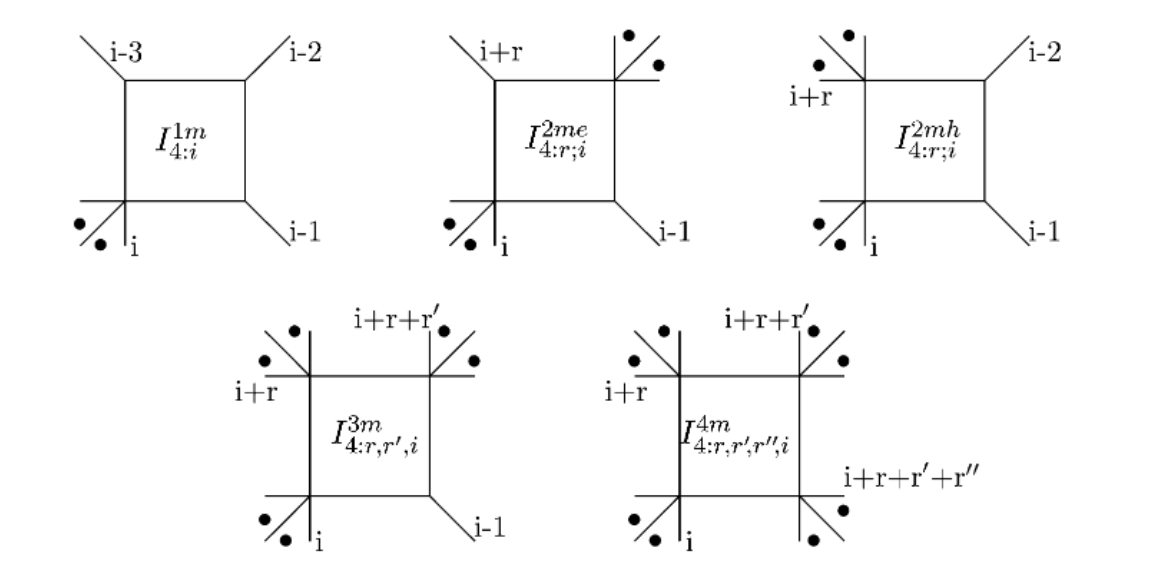
\includegraphics[width=0.8\linewidth]{box-types}
	\caption{}
	\label{fig:box-types}
\end{figure}
as well as the simplest example the zero mass integral
 \begin{figure}[H]
 	\centering
 	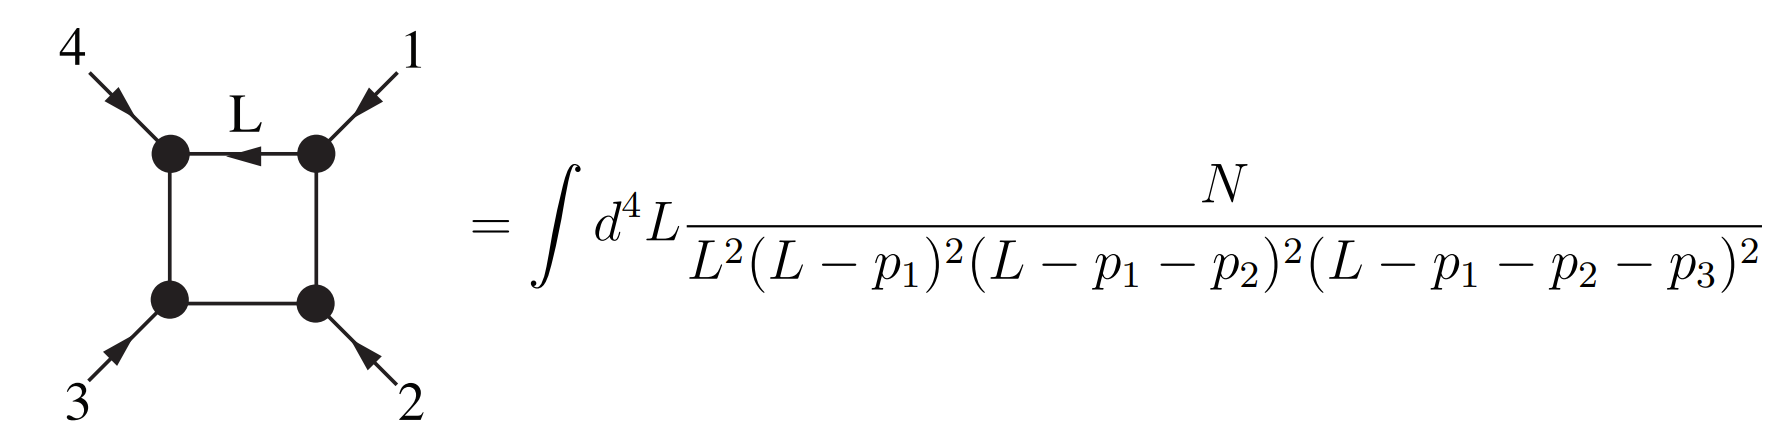
\includegraphics[width=0.9\linewidth]{zeromass}
 	\caption{}
 	\label{fig:zeromass}
 \end{figure}
where $N=(p_1+p_2)^2(p_3+p_4)^2$ is a normalization factor which we will soon see to be convenient.

We{\tiny  can define each momenta as a difference between two spacetime points
\begin{equation}
	\begin{aligned}
		p_a\equiv x_a-x_{a-1}
	\end{aligned}
\end{equation}
where each variable obeys the symmetry $x_a\to x_a+y$ leaving momentum conservation invariant $\sum p_a\to \sum p_a$. 

Further we then also have 
\begin{equation}
	\begin{aligned}
		(x_b-x_a)^2=(p_a+\cdots +p_{b-1} )^2=s_{a\cdots b-1}
	\end{aligned}
\end{equation}

One can relate null rays and points in an auxiliary space, known as twistor space using something known as the incidence relation:
\begin{equation}
	\begin{aligned}
		\mu_{\underline{\dot{\alpha}}}=x_{\underline{\alpha}\underline{\dot{\alpha}}}\lambda^{\underline{\alpha}}
	\end{aligned}
\end{equation} 
where the twistor then is 
\begin{equation}
	\begin{aligned}
		Z=(\lambda,\mu)
	\end{aligned}
\end{equation}}
\\\\
\textit{discussion of twistors}
\\\\
When discussing propagators, it is natural to see quantities of the form
\begin{equation}
	\begin{aligned}
		p_I^2=(x_a-x_c)^2
	\end{aligned}
\end{equation}
with $I=\{a,c\}$. Say that the lines $x_a$ and $x_c$ are related to the twistors $Z_A,Z_B$ and $Z_C,Z_D$ respectively. Then one can write
\begin{equation}
	\begin{aligned} \label{eq:incidence}
		(x_a-x_c)^2=\frac{\la Z_A Z_B Z_C Z_D\ra}{\la A B\ra \la C D\ra }
	\end{aligned}
\end{equation}
We can now in two steps go to first the dual coordinates $x_a$ and then the twistor coodinates. First take $L=x-x_4$. Then it follows that
\begin{equation}
	\begin{aligned}
		(L-p_1)&=([x-x_4]-[x_1-x_4])=(x-x_1)\\
		(L-p_1-p_2)&=([x-x_1]-[x_2-x_1])=(x-x_2)\\
		(L-p_1-p_2-p_3)&=([x-x_2]-[x_3-x_2])=(x-x_3)\\
		(p_1+p_2)&=([x_1-x_4]+[x_2-x_1])=(x_2-x_4)
		\\
		(p_2+p_3)&=([x_2-x_1]+[x_3-x_2])=(x_3-x_1)\\
		\dv{L}{x}&=1
		\end{aligned}
\end{equation}
which leads to
\begin{equation}
	\begin{aligned}
\int \dd^4 x	\frac{	(x_3-x_1)^2(x_2-x_4)^2}{(x-x_1)^2(x-x_2)^2(x-x_3)^2(x-x_4)^2}
	\end{aligned}
\end{equation}
When translating this integral to twistor space we get a Jacobian
\begin{equation}
	\begin{aligned}
	\int	\dd^4 x = \int \frac{\dd^4 Z_A \dd^4 Z_B}{\text{Vol}(GL(2))\times \la A B \ra^4} \equiv \int_{AB}\frac{1}{\la A B \ra^4}
	\end{aligned}
\end{equation}
as we will see, for $\mathcal{N}=4$ at one-loop we only have boxes and the factor $\frac{1}{\la A B \ra^4}$ cancels. 

Now identifying $x$ with $Z_A$ and $Z_B$ and using the association
\begin{equation}
	\begin{aligned}
		x_a\leftrightarrow (Z_a,Z_{a+1}),
	\end{aligned}
\end{equation}
we get, using \eqref{eq:incidence},
\begin{equation}
	\begin{aligned}
		(x-x_1)^2 & = \frac{\la A B 1 2\ra}{\la A B\ra \la 1 2\ra },\quad
		(x-x_2)^2 = \frac{\la A B 2 3\ra}{\la A B\ra \la 2 3\ra },\\
		(x-x_3)^2 & = \frac{\la A B 3 4\ra}{\la A B\ra \la 3 4\ra }, \quad
		(x-x_4)^2 = \frac{\la A B 4 1\ra}{\la A B\ra \la 4 1\ra },\\
		(x_3-x_1)^2 & = \frac{\la 3 4 1 2\ra}{\la 34\ra \la  1 2\ra }, \quad \,	(x_2-x_4)^2 = \frac{\la 2 3 4 1\ra}{\la 23\ra \la  4 1\ra }, 
	\end{aligned}
\end{equation}
which gives
\begin{equation}
	\begin{aligned}
		\int_{A B} \frac{\la 1234 \ra^2}{
			\la A B 1 2\ra
			\la A B 2 3\ra
			\la A B 3 4\ra
			\la A B 4 1\ra}
	\end{aligned}
\end{equation}
Let us compute the residue over $Z_A$ for $\la AB 12 \ra =0$. Schematically the four-brackets contract using the four term Levi-Cevita symbol, so the residue on $\la AB 12 \ra =0$ us found by setting $B$ equal to either $1,2$, or $A$ in the remaining brackets depending on which gives a non-zero result, i.e.,
\begin{equation}
	\begin{aligned}
		\int_{A} \frac{\la 1234 \ra^2}{
			\la A 1 2 3\ra
			\la A 2 3 4\ra
			\la A 2 4 1\ra}
	\end{aligned}
\end{equation}
Then taking the residue on $\la A 1 2 3\ra=0$ we obtain
\begin{equation}
	\begin{aligned}
	 \frac{\la 1234 \ra^2}{
			\la 1 2 3 4\ra
			\la 3 2 4 1\ra}=-1
	\end{aligned}
\end{equation}
where we have used the anti-symmetric symbol in the last line. I.e. we have a unit leading singularity when we set the maximum (2 in this case) amount of propagators on-shell.

Let us look at the 4-mass box. We are going to ignore the normalization factors in the numerator since these only depend on external kinematics. Note that while we can collect the external legs in each corner to emulate a massive particle, the internal propagators are all still massless.
 \begin{figure}[H]
	\centering
	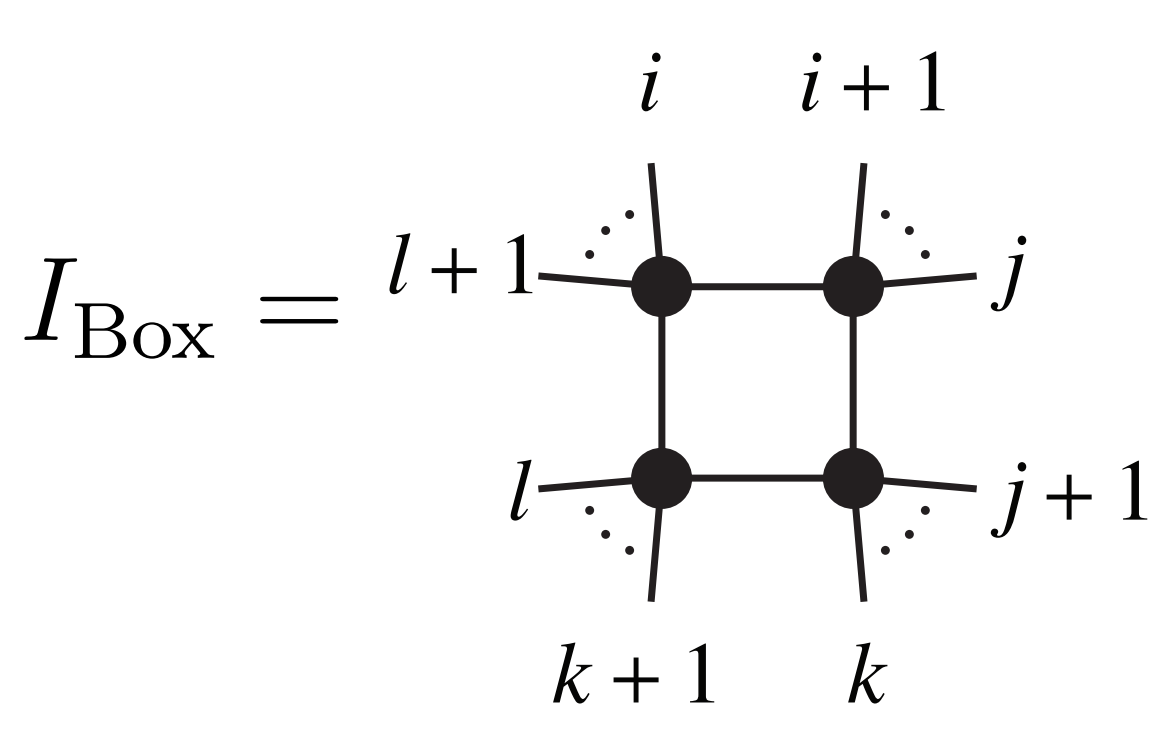
\includegraphics[width=0.4\linewidth]{fourmass}
	\caption{}
	\label{fig:fourmass}
\end{figure}
Defining $P_i\equiv p_i+\cdots+p_{l+1}$ etc, as well as $L=x-x_l$ the formula is
\begin{equation}
	\begin{aligned}
		I & = \int \dd^4 L\, \frac{1}{L^2(L-P_i)^2(L-P_i-P_j)^2(L-P_i-P_j-P_k)^2}\\
		& = \int \dd^4 x\, \frac{1}{(x-x_i)^2(x-x_j)^2(x-x_k)^2(x-x_l)^2}\\
		& = \int_{A B}\frac{1}{\la A B \ra^4}\times \frac{\la AB \ra^4\la i\,i+1 \ra \la j\,j+1 \ra \la k\,k+1 \ra \la l\,l+1 \ra}{\la A B i\,i+1 \ra \la A B j\,j+1 \ra \la A B k\,k+1 \ra \la A B l\,l+1 \ra}\\
		& = \int_{A B} \frac{\la i\,i+1 \ra \la j\,j+1 \ra \la k\,k+1 \ra \la l\,l+1 \ra}{\la A B \,i\,i+1 \ra \la A B \,j\,j+1 \ra \la A B\, k\,k+1 \ra \la A B\, l\,l+1 \ra}
	\end{aligned}
\end{equation}
It turns out that the box expansion reproduces all one-loop amplitudes post- integration, it does not match the full structure of the actual loop integrand. Here one has to also include \textit{pentagons}

\end{document}
